\chapter{Vista de proceso}
El objetivo de esta vista es mostrar que hace el sistema en alto nivel y toma en cuenta alguno de los ya citados requisitos no funcionales como es el rendimiento y la disponibilidad. Se describen tareas, sus interacciones y configuraciones, y la asignaci\'on de objetos del dise\~no y clases a las tareas. 
Este tipo de vista es fundamental para sistemas en el que el grado de concurrencia es elevado.
La arquitectura de procesos se describe en varios niveles de abstracci\'on donde cada uno de ellos tienen una funci\'on determinada.

\section{Diagramas de actividad}

Los siguientes diagramas de actividad muestra el comportamiento del sistema según las peticiones del usuario

\begin{figure}
	\centering
	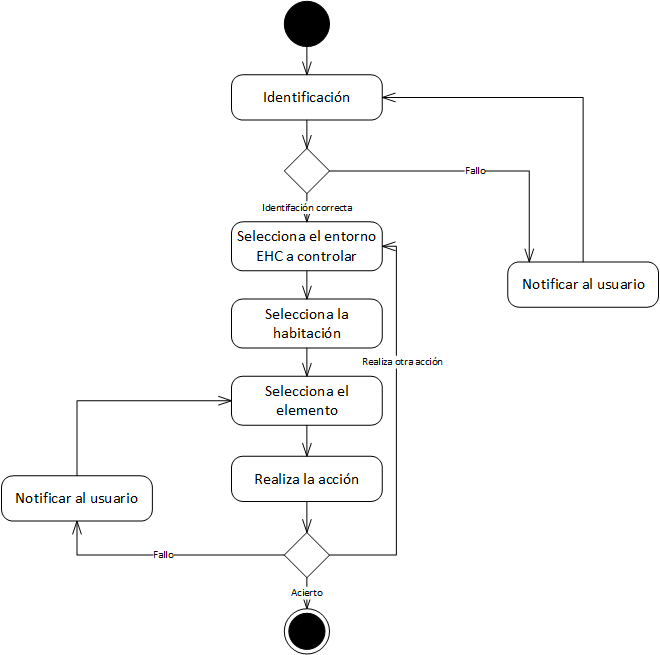
\includegraphics[width=0.65\textwidth]{4.Disenio/Imagenes/ACT-Accion}
	\caption{Diagrama de actividad: realizar una accion.}
	\label{fig:diagramaAccion}
\end{figure}

\begin{figure}
	\centering
	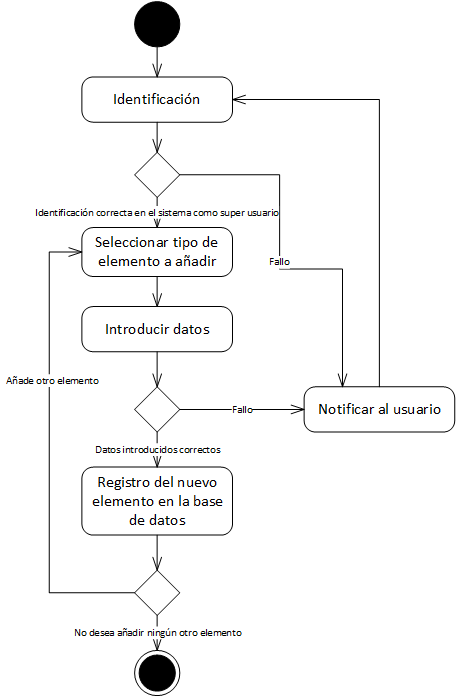
\includegraphics[width=0.65\textwidth]{4.Disenio/Imagenes/ACT-Alta}
	\caption{Diagrama de actividad: dar de alta.}
	\label{fig:diagramaAlta}
\end{figure}

\begin{figure}
	\centering
	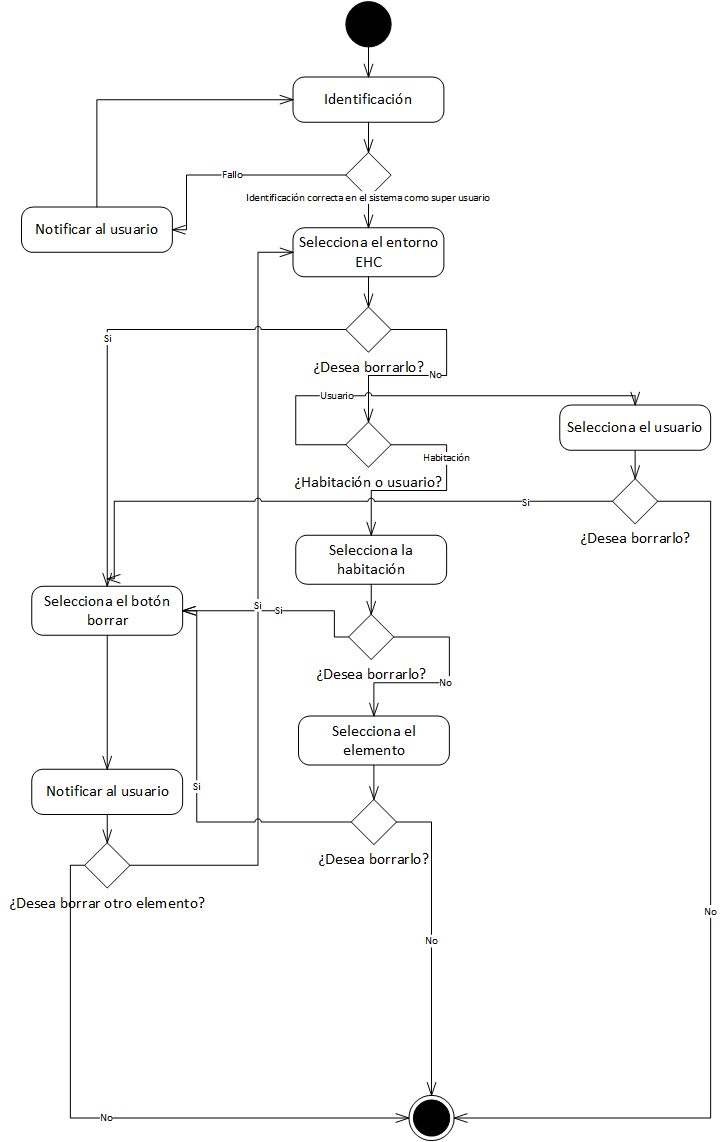
\includegraphics[width=0.65\textwidth]{4.Disenio/Imagenes/ACT-Borrar}
	\caption{Diagrama de actividad: borrar un elemento.}
	\label{fig:diagramaBorrar}
\end{figure}

\begin{figure}
	\centering
	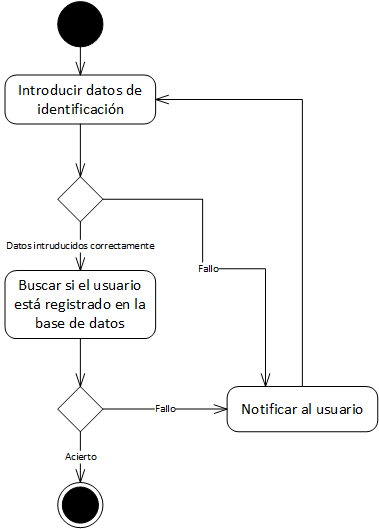
\includegraphics[width=0.65\textwidth]{4.Disenio/Imagenes/ACT-Login}
	\caption{Diagrama de actividad: identificación en el sistema.}
	\label{fig:diagramaLogin}
\end{figure}